\chapter{Reinforcement Learning Preliminaries}
This chapter is dedicated to present a concise theory of reinforcement learning. The first section will show how a certain goal can be formalized as a reward maximization -- one of the ideas which serves as a basic foundation of \ac{RL}. Section \ref{sec:mdp} explains the basics of \ac{MDP}, a general framework used in \ac{RL} problem. The notion of value function will be discussed in Section \ref{sec:value}. Subsequently, a method to solve \ac{RL}, namely policy and value iteration will be developed in section \ref{sec:value_iter}. Finally, Section \ref{sec:actor} will discuss the actor-critic structure which is an alternative solution to policy iteration.

\section{Goal as Cost Minimization}
The nature of \ac{RL} is inspired by the way living organisms learn to reach their desired goals. Animals for instance, learn by first acting on the environment, observe the changes that occur, and improve their action iteratively. One example is a circus lion that is tasked to perform acrobatic show while its trainer observing the progress. If the lion successfully executes the task, it will be rewarded with foods. Conversely, punishment will be inflicted whenever it fails. The lion initially has no idea of how to perform the task. However through trial and error, it will follow its instinct to increase the frequency of receiving rewards while trying its best to avoid punishments. In a certain duration of training, the circus lion will be finally able to perform the task flawlessly. 

Now we will formalize above illustration for robotics application. A robot can be described by its states $x_k$ with subscript $k$ denoting time instance. Applying an action $u_k$ will bring the robot to state $x_{k+1}$ with immediate reward $r_{k+1}$. Subsequently, at $k+1$ the robot applies $u_{k+1}$ which yields state $x_{k+2}$ and $r_{k+2}$. This action-state-update iteration is run for infinite time instances. The goal is defined as maximization of cumulative reward the robot receives. In control engineering, reward is usually replaced with cost. In that case the goal is defined as minimization problem. Starting from now, we will define goal as minimization of future cost $J$.

From the sequence of cost obtained over time, we can define a formalization of goal, called expected return. Return $J_t$ is a function that maps the sequence of costs into real number. An example of return is the sum of the costs:

\begin{equation}
J_t = r_{t+1} + r_{t+2} + r_{t+3} + \dots + r_T
\end{equation} 

\section{Markov Decision Process} \label{sec:mdp}
\ac{MDP} is defined as a tuple $\left<X, U, f, \rho \right>$ which satisfies Markov property \cite{babuskaRL}. The detailed explanation of Markov property can be found on \cite{sutton1998reinforcement} section 3.5 but the main idea is that to determine the probability of a state at certain time, it is sufficient to only know the state of previous time instance. The elements of the tuple are:
\begin{itemize}
	\item $X$ is the state space
	\item $U$ is the action space
	\item $f :X \times U \rightarrow X$ is the state transition function (system dynamics) 
	\item $\rho:X \times U \rightarrow \mathbb{R}$ is the reward function
\end{itemize}

In control engineering, $f$ represents the system dynamics which is a transition function mapping a current state and action to the one-step ahead state up to a probability distribution. This probability distribution is mathematically denoted as

\begin{equation}
	\text{Pr}\{x_{t+1} = x', r_{t+1} = r| x_t, u_t \}
	\label{eq:markov}
\end{equation}
where $x$ denotes state, $u$ denotes action, and $r$ denotes immediate reward obtained upon applying the input on the corresponding state. 



\section{Value Function} \label{sec:value}
Value function describes how good a particular state or state-action pair under a certain policy. As previously explained, in this thesis we will stick to control engineering convention by seeing \ac{RL} as cost minimization problem. Therefore, the smaller value function of a state $x$, the better it is. The value function is denoted by $ V^{\pi}(x) $ for state-value function and $ Q^{\pi}(x,u) $ for action-value function. Furthermore, one can always find a policy which gives an optimal value function $V^*$. This optimal value function respects the Bellman optimality equation, which can be written as 
\begin{equation}
V^*(x) = \rho(x,u) + \gamma \min_{u} V^*(f(x,u))
\label{eq:bellman}
\end{equation}
Similarly, the action-value function

\begin{equation}
Q^*(x,u) = \rho(x,u) + \gamma \min_{u} Q^*(f(x,u),u')
\label{eq:bellman2}
\end{equation}

Discount factor $\gamma$ is introduced to avoid the value function goes to infinity. Once $V^*$ is known, the optimal policy can be taken in a greedy way as
\begin{equation}
\pi^* = \text{arg} \max_{\pi} V^*(x)
\label{eq:optPi}
\end{equation}
This concludes the formulation of \ac{RL} problem. The subsequent sections will deal with two methods to solve for the solution.

\section{Policy and value iteration} \label{sec:value_iter}
The optimal policy can be reached asymptotically by means of iteration. Let initial policy be given by $ \pi_i(x,u) $. Then a new policy can be determined by first evaluating the value of $ \pi_i $ and recursively calculate the new policy $ \pi_{i+1} $. This process can be casted as an iteration algorithm as follows.

\begin{algorithm}[H]
%	\KwData{this text}
%	\KwResult{how to write algorithm with \LaTeX2e }
	\textbf{Initialization:} Start from an admissible policy $ \pi_{i} $\\
	\For{i = 1 to N}{
	\textbf{Policy Evaluation:} \\
	$ V_{i+1}(x_t) = \rho(x_t, \pi_i(x_t)) +\gamma V_{i+1}(x_{t+1}) $ \\
	
	\textbf{Policy Iteration:} \\
	$ \pi_{i+1}(x_t) = arg \min_{\pi} (\rho(x_t, \pi(x_t)) +\gamma V_{i+1}(x_{t+1})) $ \\	
	}
\caption{Policy iteration algorithm}
\end{algorithm}

The prove of iteration above is provided in \cite{Bertsekas}. In order to increase computational efficiency, instead of evaluating value function $V$ for all possible state $x$ in every iteration, one can formulate a value function evaluation recursively. The policy iteration above is then modified as shown in Algorithm \ref{algorithm2}. It can be guaranteed that $V_i$ will eventually converge to $V^*$.

\begin{algorithm}[H]
	%	\KwData{this text}
	%	\KwResult{how to write algorithm with \LaTeX2e }
	\textbf{Initialization:} Start from admissible policy $ \pi_{i} $\\
	\For{i = 1 to N}{
		\textbf{Value Iteration:} \\
		$ V_{i+1}(x_t) = \rho(x_t, \pi_i(x_t)) +\gamma V_{i}(x_{t+1}) $ \\
		
		\textbf{Policy Iteration:} \\
		$ \pi_{i+1}(x_t) = arg \min_{\pi} (\rho(x_t, \pi(x_t)) +\gamma V_{i+1}(x_{t+1})) $ \\	
	}
	\label{algorithm2}
	\caption{Value iteration algorithm}
\end{algorithm}

This type of method to find solution to \ac{RL} is called \ac{DP}. This method is closely related with a branch of control system, namely optimal control.
 
\section{Actor Critic Methods} \label{sec:actor}
The second method for solving \ac{RL} is by using temporal-difference learning. It is favored due to its model-free nature. In this section, we will discuss a class of \ac{TD} called actor-critic method. The idea of actor-critic structure is to separate policy and value function into called actor and critic entity respectively (see Figure \ref{fig:actorCritic}). These actor $\psi$ and critic $\theta$ function are parameterized by function approximators and updated using the temporal difference signal $\delta$ in every iteration. The actor-critic method is presented in Algorithm \ref{alg:actorcritic} (adapted from \cite{babuskaRL}). Note that $\tilde{u}$ denotes random exploration term.

\begin{figure}[h!]
\centering
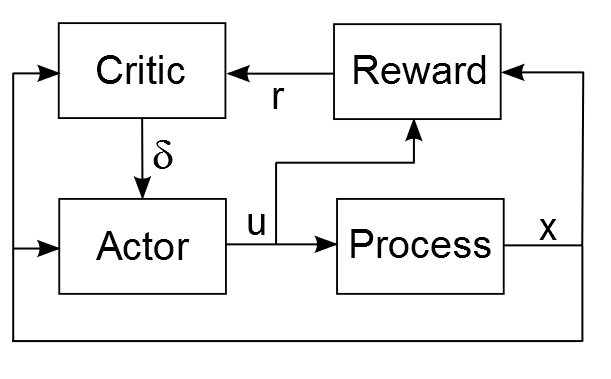
\includegraphics[width=0.6\linewidth]{actorCritic2}
\caption{Actor critic structure} 
\label{fig:actorCritic}
\end{figure}

\begin{algorithm}[H]
	\For{every trial}{
		Initialize $x_0$ and $u_0 = \tilde{u}_0$\\
		\Repeat{terminal state}{
			apply $u_k$, measure $x_{k+1}$, receive $r_{k+1}$ \\
			choose next action $ u_{k+1} = \hat{\pi}(x_{k+1}, \psi_k)	+ \tilde{u}_{k+1} $ \\
			$ \delta_k = r_{k+1} + \hat{V}(x_{k+1}, \theta_k) - \hat{V}(x_{k}, \theta_k) $ \\
			$ \theta_{k+1} = \theta_k + \alpha_c\delta_k \frac{\partial \hat{V}(x,\theta)}{\partial \theta} \bigg|_{x=x_k, \theta = \theta_k}$ \\
			$ \psi_{k+1} = \psi_k + \alpha_c\delta_k \frac{\partial \hat{V}(x,\psi)}{\partial \psi} \bigg|_{x=x_k, \psi = \psi_k}$
		}
	}
	\label{alg:actorcritic}
	\caption{Actor-critic algorithm}
\end{algorithm}



